\documentclass[12pt,a4paper]{article}
%\usepackage[a4paper, total={6in, 8in}]{geometry}
\usepackage{geometry}
 \geometry{
 top=25mm,
 }
%\usepackage[showframe]{geometry}
\usepackage[english]{babel}
\usepackage[T1]{fontenc}
\usepackage{mathptmx}
%\usepackage{newtxmath,newtxtext}
%\usepackage[utf8x]{inputenc}
\usepackage{amsmath}
\usepackage{graphicx}
\graphicspath{ {images/} }
\usepackage[colorinlistoftodos]{todonotes}
\usepackage[yyyymmdd]{datetime}
\usepackage{tikz}
\usetikzlibrary{calc}
\usepackage{sectsty}
\usepackage{float}
%\usepackage[table,xcdraw]{xcolor}
\sectionfont{\fontsize{18pt}{15}\selectfont}
\usepackage{tocloft}
\renewcommand{\cftsecleader}{\cftdotfill{\cftdotsep}}

\begin{document}
\pagenumbering{roman}
\tableofcontents
\newpage
\pagenumbering{arabic}
\setcounter{page}{1}
%\addcontentsline{toc}{section}{Unnumbered Section}
\section{\textbf{Problem Statement}}
Return a random paragraph generated from sentences populated by semi-pronounceable random (nonsense) words. ... random-title - Return a random title populated by semi-pronounceable random (nonsense) words. random-sentence - Return a random sentence populated by semi-pronounceable 






\section{\textbf{Overall Architecture}} 

\begin{figure}[h]
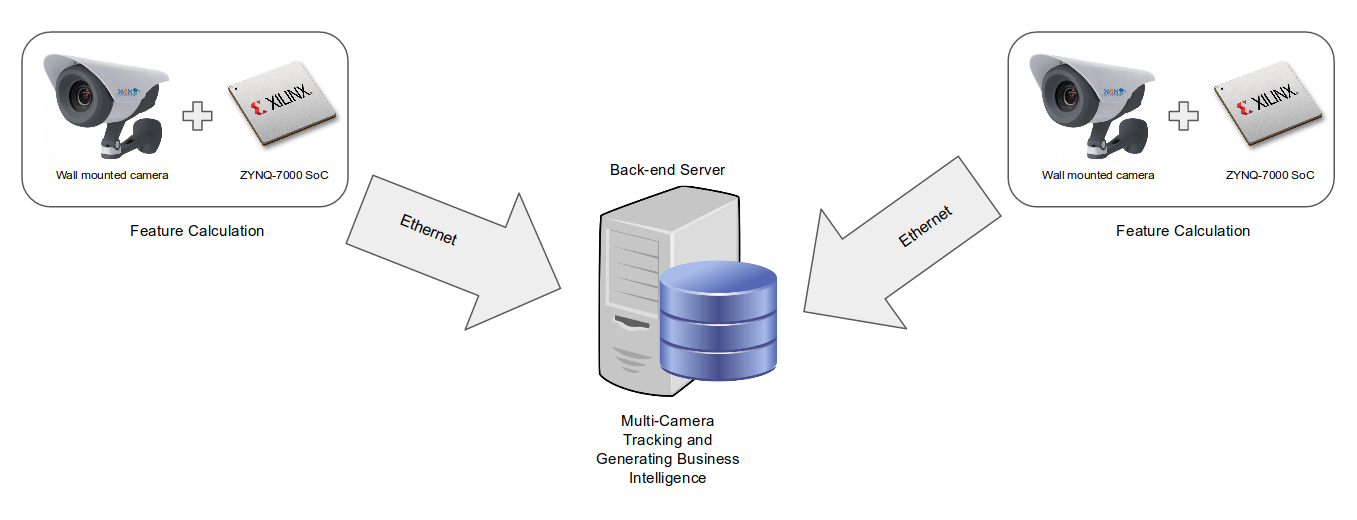
\includegraphics[width=10cm]{architecture.png}
\centering
\caption{Overall architecture of the system}
\label{f2}
\end{figure}



\newpage
%\section*{\textbf{References}}
\addcontentsline{toc}{section}{References}
\begin{thebibliography}{7}

\bibitem{1}
Vicente, Alfredo Gardel, et al. "Embedded vision modules for tracking and counting people." \textit{IEEE Transactions on Instrumentation and Measurement} 58.9 (2009): 3004-3011.

\bibitem{2}
Dalal, Navneet, and Bill Triggs. "Histograms of oriented gradients for human detection." Computer Vision and Pattern Recognition, 2005. CVPR 2005. \textit{IEEE Computer Society Conference on}. Vol. 1. IEEE, 2005.

\end{thebibliography}


\end{document}